\documentclass[12pt]{article}
\usepackage{graphicx,amssymb}

\oddsidemargin  -0.5 cm
\evensidemargin 0.0 cm
\textwidth      6.5in
\headheight     0.0in
\topmargin      -1 cm
\textheight=9.0in

\begin{document}

\begin{flushright}
  Jim Pivarski
\end{flushright}

\section*{Prologue: What is Quantum Field Theory?}

Quantum Field Theory (QFT) is the modern paradigm for theories of
particle physics: it's not a specific model for how the world works
and what things are in it; it is the mathematical structure in which
new theories are proposed.  It's on a more basic level, therefore,
than a theory like the Standard Model.  The Standard Model tries to
encapsulate all known data into a single Lagrangian (a function that
I'll define later), but QFT is the machinery that tells us what to do
with that Lagrangian to make predictions.

The subject of Quantum Field Theory splits nicely into two conceptual
parts: ``quantum'' and ``field.''  I'll first talk about quantum as
opposed to classical mechanics, then about field as opposed to
classical theories.

Summary of the differences between classical and quantum:
\begin{center}
  \begin{tabular}{p{0.4\linewidth} | p{0.4\linewidth}}
    classical & quantum \\\hline
    $\bullet$ specify initial or boundary conditions (which are
    measured) & $\bullet$ specify boundary conditions (which are
    measured) \\
    $\bullet$ predict future or intermediate region of space &
    $\bullet$ under certain conditions, the intermediate region is
    inaccessible to measurements, so you don't {\it predict} anything
    at all about it \\
    $\bullet$ measure to see if you're right! & $\bullet$ predict
    probability of the process (the final state given the initial
    state); count to see if you're right!
  \end{tabular}
\end{center}

Summary of the differences between particle and field:
\begin{center}
  \begin{tabular}{p{0.4\linewidth} | p{0.4\linewidth}}
    particle mechanics & field theory \\\hline
    $\bullet$ parameterized curves follow point particles around
    (geodesics on a manifold) subject to equations of constraint &
    $\bullet$ a function defined over all space evolves according to a
    PDE \\
    $\bullet$ 3 $\times$ $N$ degrees of freedom & a continuum of
    degrees of freedom?  (perhaps only countable, as non-zero
    measurement error makes functions with pointwise differences
    equivalent) \\
    $\bullet$ the number of particles is built into the theory &
    $\bullet$ what are particles? \\
    $\bullet$ dynamics comes from forces, which are the equations of
    constraint & $\bullet$ dynamics comes from interactions between
    fields, which are terms in the PDE (cello string $f(x)$, air
    pressure $\rho(\vec{x})$)
  \end{tabular}
\end{center}

While we're at it, we should know about that other dichotomy of modern
physics:
\begin{center}
  \begin{tabular}{p{0.4\linewidth} | p{0.4\linewidth}}
    non-relativistic & relativistic \\\hline
    $\bullet$ kinetic energy is $E = \frac{1}{2} mv^2 =
    \frac{p^2}{2m}$ & motion energy is $E = \sqrt{p^2c^2 + m^2c^4}$ \\
    & (when $p \ll m$, $E \approx mc^2 + \frac{p^2}{2m}$) \\
  \end{tabular}
\end{center}

Because I would forget to include them otherwise, we choose units in
which $c = \hbar = 1$.  $c = 1$ defines natural units for relativity,
in which length and time have the same units; $\hbar = 1$ defines
natural units for quantum mechanics, in which energy and length have
inverse units.

\section{Introduction to Quantum Mechanics with Feynman-Dirac Path Integrals}

\begin{center}
  \includegraphics[width=0.6\linewidth]{fig1.eps}
\end{center}
Phenomenon of classical waves: light through two slits makes an
interference pattern.
\begin{equation}
  \left( \frac{\partial^2}{\partial t^2} - \nabla^2 \right) A = 0
  \mbox{ has solutions } A = exp(i\omega t - \vec{k} \cdot \vec{x})
  \mbox{ with } \omega^2 = |\vec{k}|^2
\end{equation}
\begin{equation}
  \mbox{intensity of light on screen } = I = \int_{\mbox{\scriptsize
  one period}} dt \, A(t, \vec{x}_{\mbox{\scriptsize screen}})^*
  A(t, \vec{x}_{\mbox{\scriptsize screen}})
\end{equation}

Difference in phase of light from the two paths is
\begin{equation}
  2 \pi d / \lambda \mbox{ where $\lambda$ is wavelength: } \lambda \omega = 2 \pi c
\end{equation}
where we assume that $d \ll D$ (we will use this assumption again later!)

Surprise: light comes in particles in the sense that we can release
one at a time.  (We will understand why at the very end of this
lecture.)  What happens to the interference pattern if you {\it do}
release ``photo-ons'' one at a time?  (Answer: the same pattern, but
the intensity is a histogram of events accumulated for a large number
of photons.)  How can this be explained in (local) particle mechanics?
\begin{center}
  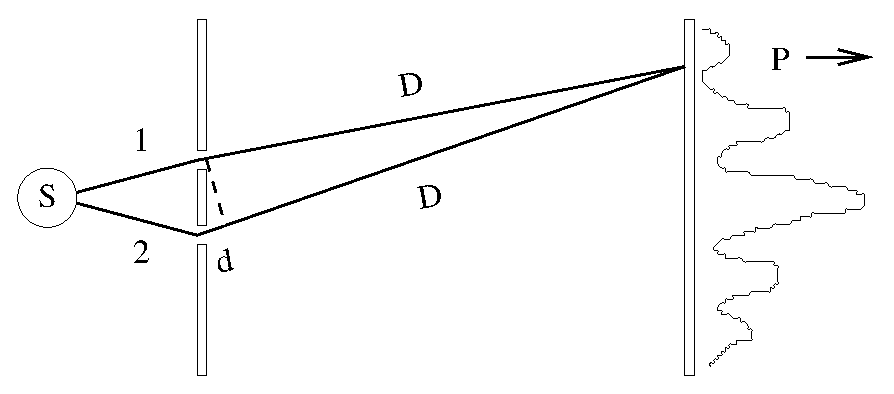
\includegraphics[width=0.6\linewidth]{fig2.eps}
\end{center}

Weird geodesic of crooked line through slit is okay in principle, but
when the other hole is covered, the pattern disappears (replaced with
spot).  Both paths somehow contribute.  Suppose there's an analogy of
``phase difference.''

The right hypothesis is that the ``pseudo-phase'' of a path (not a
point on the path, but a path) is the action.
\begin{center}
  \begin{tabular}{p{0.45\linewidth} p{0.35\linewidth}}
    Epitome of nineteenth-century physics: \\\hline
    $\bullet$ Lagrangian $\mathcal{L}$ characterizes system & $\mathcal{L}(x,
    \partial x / \partial t) =$ kinetic energy $-$ potential energy \\
    $\bullet$ action $S$ & $\displaystyle S(x, \partial x / \partial t) = \int_0^T dt \,
    \mathcal{L}$ \\
  \end{tabular}
\end{center}
In classical physics, the action is a functional of the system which
is minimized by the true evolution of the system.  This means that we
treat $x$ and $(\partial x / \partial t)$ as two independent variables
and apply the Euler-Lagrange solution:
\begin{equation}
  \frac{d}{dt} \left( \frac{\partial \mathcal{L}}{\partial (\partial x
  / \partial t)} \right) - \frac{\partial \mathcal{L}}{\partial x} = 0
\end{equation}
A classical Lagrangian for free particles: $\mathcal{L} = \frac{1}{2}
m (\partial x / \partial t)^2$ is minimized by $\frac{d}{dt} \left( m
(\partial x / \partial t) \right) = 0$, constant velocity
(straight-line) motion.

(The unitless phase is actually $S/\hbar$, where $S$ and $\hbar$ have
the same units: action.  $\hbar$ is a very small unit of action:
phases can only differ in observable ways for very small actions.  But
$\hbar$ is 1.)

Action of path 1: $\displaystyle S = \int_0^T dt \, \frac{1}{2} m
(\partial x / \partial t)^2 = \frac{1}{2} m (\partial x / \partial
t)^2 T = \frac{m}{2} \left(\frac{D}{T}\right)^2 T$

\smallskip

Action of path 2: $\displaystyle S = \int_0^T dt \, \frac{1}{2} m
(\partial x / \partial t)^2 = \frac{1}{2} m (\partial x / \partial
t)^2 T = \frac{m}{2} \left(\frac{D + d}{T}\right)^2 T$

Pseudo-phase difference is $m D d / T \hbar$.

DeBroglie hypothesis: $p = h / \lambda = 2 \pi \hbar / \lambda$ and $p
= m D / T$

So the pseudo-phase difference is really $2 \pi d / \lambda$.

What if there are two screens?  (Then there are four paths
superimposing.)  What if there are three slits?  (Then there are three
paths.)  What if there are infinitely many screens with infinitely
many slits ($=$ nothing at all)?  All possible paths contribute to the
detected pattern: a sum of $e^iS$ is performed over all possible paths
and the absolute magnitude squared is the probability.

New paradigm: we are no longer trying to predict what happens to the
particle between the source and the screen--- the emission and
detection are the only measurements made in this experiment.  (If
additional interactions are added to make measurements in the middle,
the pattern changes.)  We also now have probabilities between zero and
one for the likelihood of the second measurement, so that becomes the
new prediction.  What happens between measurements is an {\it
explanation} of the phenomenon, but {\it predictions} are now limited
only to the probability of the second measurement.  This is the axiom
of quantum mechanics:
\begin{equation}
  P(x_b(T) | x_a(0)) = \left| \lim_{\varepsilon \to 0} \int D[x] \exp\left( i \int_0^T
  dt (1 + i \varepsilon) \, \mathcal{L}(x, \partial x / \partial t)
  \right) \right|^2 = \left| \mathcal{U}(x_a, x_b, T) \right|^2
\end{equation}
where $x$ is a path parameterized by $t$: $x(t)$ such that $x(0) =
x_a$ and $x(T) = x_b$.  $D[x]$ is a sum over all paths $x$.

Hey, aren't there $\aleph_2$ of those?

\section{How to ``Sum Over All Paths''}

Even if the Lebesgue measure doesn't exist, you can define integrals
by Riemannian sums.  Divide $T$ into short timesteps of length $a$.  A
path $x$ is then characterized by a finite sequence $\{x_1, x_2, x_3,
\ldots x_N\}$ in which the $x_k$'s can be anything.  (The particle can
go to Andromeda and back between timesteps.  This is okay for two
reasons: the theory we're working with is non-relativistic, but more
importantly, the theory only predicts the probability of this process.
If we were to ask a different question with a relativistic theory, all
probabilities of influence on Andromeda are zero.)

Now we can define a prescription for summing (integrating) over all
these paths:
\begin{center}
  \begin{tabular}{p{0.55\linewidth} p{0.35\linewidth}}
    \begin{minipage}{\linewidth}
      \[ \int D[x] = \frac{1}{C(a)} \int_{-\infty}^\infty \frac{dx_1}{C(a)} \int_{-\infty}^\infty
      \frac{dx_2}{C(a)} \ldots \int_{-\infty}^\infty
      \frac{dx_N}{C(a)} \]
      $x_a$ and $x_b = x_N$ are endpoints.
    \end{minipage} &
    \begin{minipage}{\linewidth}
      \includegraphics[width=\linewidth]{fig3.eps}
    \end{minipage}
  \end{tabular}
\end{center}

On a lattice, derivatives become finite differences, so
\begin{equation}
  \int_0^T dt \, \mathcal{L}(x, \frac{\partial x}{\partial t}) =
  \int_0^T dt \, \left( \frac{1}{2} m \left(\frac{\partial x}{\partial t} \right)^2 - V(x)
  \right) \to
  \sum_{k=0}^N \left( \frac{1}{2} m \frac{(x_{k+1} - x_k)^2}{a} - a
  V(x) \right)
\end{equation}

After evaluating all the integrals, we take a limit $a \to 0$ which
makes $\mathcal{U}$ is continuous; that is, we'll choose $C(a)$ such
that
\begin{equation}
  \lim_{a \to 0} \bigg( \mathcal{U}(x_a, x_b, T) - \mathcal{U}(x_a,
  x_b, T - a) \bigg) = 0
\end{equation}

Nomenclature: I call $x$, which is measurable at the endpoints, a
dynamical variable--- the physics information.  I call $t$ a parameter
because it is the parameter of the curves $x(t)$.  The parameters are
discretized into a lattice, and the values of the dynamical variables
are integrated over.

\section{Deriving the Schr\"odinger Equation}

\label{sec:schrodinger}

There are at least three equivalent formulations of quantum mechanics,
I've picked as an introduction the last to be discovered, the last to
be taught to physics majors, and the favorite of many of today's
theorists.  The first to be discovered, the first to be taught to
physics majors, and the one which is generally ignored by today's
theorists is the Schr\"odinger equation.  (The third is the one
physicists know best, but you won't see any bras or kets in this
talk.)

The Schr\"odinger equation is a PDE of $\psi(x;t)$, a complex function
over both dynamical variables and parameter.  It is interpreted as a
distribution of uncertainty in $x$ between measurements: for a
measurement of $x$ at time $t$,
\begin{equation} 
  \int_{x-\Delta x}^{x+\Delta x} dx \, |\psi(x;t)^* \psi(x;t)|^2
\end{equation}
is the probability that the particle will be found in a region
$(x-\Delta x, x+\Delta x)$.  Schr\"odinger's equation describes the
evolution of this uncertainty with time.
\begin{equation}
  i \frac{\partial}{\partial t} \psi(x;t) = \left(
  -\frac{1}{2 m} \frac{\partial^2}{\partial x^2} + V(x) \right)
  \psi(x;t)
  \label{eqn:schrodinger}
\end{equation}

The weird thing about Schr\"odinger's treatment is that once a
particle has been measured in a region $(x-\Delta x, x+\Delta x)$, the
function $\psi(x;t)$ {\it abruptly} changes to fill only that region
(or exclude that region if the particle was found to be not in
$(x-\Delta x, x+\Delta x)$).  I think this weirdness comes from trying
to think of quantum mechanics as an initial value problem, rather than
a boundary value problem.

Let's derive the Schr\"odinger equation from our path integral
formulation.  We'll start by only looking at the last integral:
\begin{equation}
  \mathcal{U}(x_a, x_b, T) = \lim_{\varepsilon \to 0} \int_{-\infty}^\infty \frac{dx'}{C(a)}
  \exp \left(i (1 + i\varepsilon) \left(\frac{m(x_b - x')^2}{2 a} -
  aV(x_b) \right) \right) \mathcal{U}(x_a, x', T - a)
\end{equation}
The set of all paths from $x_a$ to $x_b$ is the set from $x_a$ to $x'$
and from $x'$ to $x_b$, provided that you consider all possible $x'$s.

Because of the $(1+i\varepsilon)$ (known in other contexts as the
Feynman prescription), exponentials with large $|x_b - x'|$ will
contribute negligibly.  Let's therefore expand the $\mathcal{U}$ on
the right-hand-side in two powers of $(x' - x_b)$.  We can also factor
out the $V(x)$ term and expand that to first order in $a$ because $a$
is small.
\[
  \mathcal{U}(x_a, x_b, T) = \lim_{\varepsilon \to 0}
  \int_{-\infty}^\infty \frac{dx'}{C(a)} \exp \left(i (1 +
  i\varepsilon) \frac{m(x_b - x')^2}{2 a} \right) \left(1 - iaV(x_b)
  \right) \times
\]
\begin{equation}
  \mbox{\hspace{4.5 cm}} \times \left(1 + (x' -
  x_b)\frac{\partial}{\partial x_b} + \frac{1}{2}(x' - x_b)^2
  \frac{\partial^2}{\partial x_b^2}\right) \mathcal{U}(x_a, x_b, T - a)
\end{equation}

Again because of the $(1+i\varepsilon)$, we can evaluate these
integrals using Gaussian integration formulas.
\begin{equation}
  \int_{-\infty}^\infty d\xi \, e^{-b \xi^2} = \sqrt{\frac{\pi}{b}} \mbox{\hspace{1 cm}}
  \int_{-\infty}^\infty d\xi \, \xi e^{-b \xi^2} = 0 \mbox{\hspace{1 cm}}
  \int_{-\infty}^\infty d\xi \, \xi^2 e^{-b \xi^2} = \frac{1}{2b} \sqrt{\frac{\pi}{b}} \mbox{\hspace{1 cm}}
\end{equation}

Integrating and taking the $\varepsilon \to 0$ limit, we get
\begin{equation}
  \mathcal{U}(x_a, x_b, T) = \left(\frac{1}{C(a)} \sqrt{\frac{2 \pi
  a}{-i m}} \right) \left(1 - iaV(x_b) + \frac{ia}{2m}
  \frac{\partial^2}{\partial x_b^2} + \mathcal{O}(a^2) \right)
  \mathcal{U}(x_a, x_b, T - a)
\end{equation}
To make $\mathcal{U}$ continuous, $C(a)$ must be $\sqrt{-im/2\pi a}$.

Move the $\mathcal{U}(x_a,x_b,T-a)$ onto the left-hand-side and
multiply by $i/a$.
\begin{equation}
  i\left(\frac{\mathcal{U}(x_a,x_b,T) - \mathcal{U}(x_a,x_b,T-a)}{a} \right) =
  \left( V(x_b) - \frac{1}{2m}\frac{\partial^2}{\partial x_b^2} +
  \mathcal{O}(a^2)\right) \mathcal{U}(x_a,x_b,T-a)
\end{equation}
That looks like a derivative to me.

\begin{equation}
  i \frac{\partial}{\partial T} \mathcal{U}(x_a, x_b, T) =
  \left(\frac{1}{2m} \frac{\partial^2}{\partial x_b^2} + V(x_b)
  \right) \mathcal{U}(x_a, x_b, T)
\end{equation}
This is the Schr\"odinger equation (\ref{eqn:schrodinger}), but with
initial conditions $x_a$ built-in.  If $\psi(x;t)$ represents the
fuzziness of where a particle is, $\mathcal{U}(x_a, x_b, T)$
represents the stringyness of where a particle can go.

As an initial value problem (Schr\"odinger's formulation), uncertainty
in $x_b$ grows while you're waiting to do your second measurement.
Once you make it, the uncertainty is sharply constricted.  (What does
$\frac{\partial}{\partial T} \mathcal{U}(x_a, x_b, T)$ mean then?)  As
a boundary value problem, you consider what kind of process you'd like
to measure (particle goes from here to there), you calculate its
probability, and then you measure an ensemble.  (This is what we do in
practice, with Feynman diagrams.)  The particle spreading out all over
space in between measurements is an explanation for the interference
you see in the second measurement, but you only ever predict discrete
probabilities.  (Uncertainty is in the process, rather than the
position.)

Even though the particle's paths (or position) smear over space, and
$\psi(x;t)$ is called a ``wavefunction,'' this is still a particle
theory.  You still have a dynamical variable (or three) for every
particle in the universe, and no way to represent particle creation or
annihilation.  Since we know that nature has the freedom to create and
destroy particles, this too must be a dynamical variable.  A beautiful
if non-intuitive way to do this is to replace the particle theory for
a field theory.  We will see that when a field theory is made quantum,
non-negative integer excitations result.  These excitations of which
you can have one or two but never one and a half are particles.  The
existence of atoms was the first quantum effect discovered, but the
last to be recognized as a quantum effect.

\section{Classical Field Theory as a Space-Filling Mattress}

First, we will need a classical description of a field that we can
apply our path integral formulation to.  The particle to field
transition is like the classical to quantum transition in one respect:
we add a {\it lot} of new degrees of freedom.

Since the state of the system in a field theory is expressed by a
function $\phi(t,x,y,z)$, there is a dynamical variable for every
point in space-time.  Therefore, let's think for now of a field as a
collection of particles (I'll call them pseudoparticles to avoid
confusion with the real particles we'll get by quantizing this field)
with one particle fixed at every point in space $(x,y,z)$.  These
pseudoparticles are free to move in only one direction: a new
dimension called $\phi$.  (Or four new directions $A_0$, $A_1$, $A_2$,
$A_3$ for a field with polarizations, but we'll keep it simple.)

Because the particles cannot move in $(x,y,z)$, this becomes a
labeling scheme.  Our dynamic variables are therefore
$\phi_{(x,y,z)}(t)$, in the next section, we'll sum over paths in
$\phi$--$t$.  What dynamics we will get from such a procedure will
depend on the form of the Lagrangian.

Most wave equations have the following form: $(\partial^2/\partial t^2
- \nabla^2) \phi(t,\vec{x}) = 0$.  This can be derived from an extreme
of the Lagrangian
\begin{equation}
  \mathcal{L} = \left( \frac{\partial \phi}{\partial t} \right)^2 -
  \left( \frac{\partial \phi}{\partial x} \right)^2 - \left(
  \frac{\partial \phi}{\partial y} \right)^2 - \left( \frac{\partial
  \phi}{\partial z} \right)^2
\end{equation}
In a field theory context, the Euler-Lagrange equations contain
derivatives of fields values and field variables (treated as
independent quantities, as before).
\begin{equation}
  \frac{d}{dt} \left( \frac{\partial \mathcal{L}}{\partial (\partial \phi / \partial t)} \right) +
  \frac{d}{dx} \left( \frac{\partial \mathcal{L}}{\partial (\partial \phi / \partial x)} \right) +
  \frac{d}{dy} \left( \frac{\partial \mathcal{L}}{\partial (\partial \phi / \partial y)} \right) +
  \frac{d}{dz} \left( \frac{\partial \mathcal{L}}{\partial (\partial \phi / \partial z)} \right) -
  \frac{\partial \mathcal{L}}{\partial \phi} = 0
\end{equation}
Applying this, we get our wave equation
\begin{equation}
  \frac{d}{dt} \left(2 \frac{\partial \phi}{\partial t} \right) +
  \frac{d}{dx} \left(-2 \frac{\partial \phi}{\partial x} \right) +
  \frac{d}{dy} \left(-2 \frac{\partial \phi}{\partial y} \right) +
  \frac{d}{dz} \left(-2 \frac{\partial \phi}{\partial z} \right) - 0 = 0
\end{equation}

What's happening to our pseudoparticles?  The fact that they have
kinetic energy (the only positive term) $(\partial \phi / \partial
t)^2$ isn't surprising--- that's just like an $m=2$ non-relativistic
particle.  But the potential energy has terms like $(\partial \phi /
\partial x)^2$.  Thinking of space coordinates as particle labels,
this means that the pseudoparticles have a Hook's law potential (a
spring) between nearest neighbors.  The field is simply a massive
coupled oscillator, like a mattress filling all of space.  The fact
that the spring constant $k=2$ makes the energy cost for large $\phi$
differences between neighbors the same as the energy cost for large
$\phi$ differences in time, so waves in the oscillator system
propagate at the speed of light (1.0).

One nice thing about field theories is that they're magically
relativistic.  Our non-relativistic model of pseudoparticles,
interpreted as a field, is fully relativistic, and in fact, looks a
lot like the theory that inspired ``On the Electrodynamics of Moving
Bodies'' (1905).  We'll be quantizing a more general Lagrangian, one
that has an energy cost for having any field ($\phi \ne 0$) at all.
This is our last Lagrangian:
\begin{equation}
  \mathcal{L} = \left( \frac{\partial \phi}{\partial t} \right)^2 -
  \left( \frac{\partial \phi}{\partial x} \right)^2 - \left(
  \frac{\partial \phi}{\partial y} \right)^2 - \left( \frac{\partial
  \phi}{\partial z} \right)^2 - m^2 \phi^2
\end{equation}
This last term makes its way into the wave equation like this:
\begin{equation}
  \frac{\partial^2 \phi}{\partial t^2} - \nabla^2 \phi + m^2 \phi = 0
\end{equation}
Such an equation has solutions
\begin{equation}
  \phi(t, \vec{x}) = \exp(iEt + i\vec{p}\cdot\vec{x}) \mbox{ for
  constants $E$ and $\vec{p}$ that solve } -E^2 + |\vec{p}|^2 + m^2 = 0
\end{equation}

Perhaps we'd like to interpret an excitation in this field as a
particle.  You can heap the field together in a mound by superimposing
solutions with different $\vec{p}$ constants--- in particular, a
distribution like $exp(-|\vec{p}|^2)$ will give you a spacial
distribution like $exp(-|\vec{x}|^2)$, a Gaussian wave packet.  (Do
Fourier transforms from $\vec{p}$ to $\vec{x}$.)  This kind of
solution can sit still and has total energy (in its rest frame)
$m \int d^3x |\phi(t, \vec{x})|^2$.  Looks like a particle to me.

One very non-particulate feature of this solution, though, is that
there is no constraint on the overall amplitude of $\phi$.  If an
excitation of amplitude $\phi$ is one particle, what is an excitation
of amplitude $1.5 \phi$?

\section{Quantizing Field Theory}

Our prescription for summing over paths, rather than just picking the
smallest-action one, looks like this for fields:
\[ P(\phi_{(x,y,z)}(T) | \phi_{(x,y,z)}(-T)) = \mbox{\hspace{10 cm}} \]
\begin{equation}
  \mbox{\hspace{2 cm}} \left| \lim_{\varepsilon \to
  0} \int D[\phi] \exp\left(i \int_{-T}^T dt (1 + i \varepsilon) \,
  \int_{\mathbb{R}^3} d^3 x \, \mathcal{L}\left(\phi, \frac{\partial \phi}{\partial
  t}, \frac{\partial \phi}{\partial x}, \frac{\partial \phi}{\partial
  y}, \frac{\partial \phi}{\partial z}\right) \right) \right|^2
\end{equation}
Now $D[\phi]$ refers to a derivative over highly parametric curves
through {\it all} the pseudoparticles' paths.  Exponential factors for
each pseudoparticle have been combined to become an integral over all
space (pseudoparticles) in the exponent.  If we were budding theorists
wanting to learn how to calculate Feynman diagrams, the right thing to
do at this point would be to let $T \to \infty$ and insert factors of
$\phi(x_{\mbox{\scriptsize source}})$ and $\phi(x_{\mbox{\scriptsize
sink}})$ under the $D[\phi]$ integral to make Lorentz-invariant
correlation functions, and then develop functional derivatives and
Green's functionals to be able to do calculations.  That might sound
like fun (?), but we don't have time for it.

Let's put this integral into a form we know how to calculate.

\section{A New(?) Schr\"odinger Equation}

The quantum mechanics path integral could be turned into a
Schr\"odinger equation, so why not the quantum field theory one?  I
was not able to work through a complete derivation like the one in
Section \ref{sec:schrodinger} (sums of sums of integrals of sums), but
I wouldn't be able to present it, either.  The following is a
heuristic derivation.  If I had worked it all out properly, I would
expect the following to work anyway, as a check.

In quantum {\it mechanics} (QM), the Lagrangian $\mathcal{L}(x,
\partial x/\partial t) = (1/2) m (\partial x/\partial t)^2 - V(x)$
yielded the Schr\"odinger equation
\[ i \frac{\partial \Psi}{\partial t} = \left( -\frac{1}{2m}
\frac{\partial^2}{\partial x^2} + V(x) \right) \Psi(x;t) \]
where $x$ is the dynamical variable and $t$ is the parameter, and
$\Psi(x;t)$ describes the spreading of paths $x(t)$ between
measurements.

In QFT, we have the Lagrangian $\mathcal{L}(\phi, \partial
\phi/\partial t, \partial \phi/\partial x, \partial \phi/\partial y,
\partial \phi/\partial z) = \left( \frac{\partial \phi}{\partial t}
\right)^2 - \left( \frac{\partial \phi}{\partial x} \right)^2 - \left(
\frac{\partial \phi}{\partial y} \right)^2 - \left( \frac{\partial
\phi}{\partial z} \right)^2 - V(\phi)$ where $\phi$ is a dynamical
variable over the parameter {\it space} $(t, x, y, z)$.  Our paths
(1-D manifolds) have become bulks (4-D manifolds).  We expect a
distribution function $\Psi(\phi; t, x, y, z)$.

In QM, the squared first derivative $\partial x/\partial t$ had the
dynamical variable replaced by the distribution $\Psi$, and it was
square-rooted to become the left-hand side of the Schr\"odinger
equation.  By analogy, the left-hand side of the QFT Schr\"odinger
equation should be
\begin{equation}
  i\sqrt{\left(\frac{\partial \Psi}{\partial t}\right)^2 -
  \left(\frac{\partial \Psi}{\partial x}\right)^2 - \left(\frac{\partial
  \Psi}{\partial y}\right)^2 - \left(\frac{\partial \Psi}{\partial z}\right)^2}
\end{equation}

The right-hand side featured a second derivative of the dynamical
variable, which is now $\phi$, and we are also now missing a factor of
$m/2$.  The right-hand side should therefore be
\begin{equation}
  \left(-\frac{1}{4} \frac{\partial^2}{\partial \phi^2} + V(\phi)
  \right) \Psi(\phi; t, x, y, z)
\end{equation}

Someone who is brave enough to do the whole derivation properly can
tell me some day why the $1/4$ should really be $1/2$.  The whole
QFT Schr\"odinger equation is
\begin{equation}
  i\sqrt{\left(\frac{\partial \Psi}{\partial t}\right)^2 -
  \left(\frac{\partial \Psi}{\partial x}\right)^2 - \left(\frac{\partial
  \Psi}{\partial y}\right)^2 - \left(\frac{\partial \Psi}{\partial
  z}\right)^2} =
  \left(-\frac{1}{2} \frac{\partial^2}{\partial \phi^2} + V(\phi)
  \right) \Psi(\phi; t, x, y, z)
\label{eqn:qftschrodinger}
\end{equation}

\section{Deriving Particles from Quantum Field Theory}

Now that we have a PDE, we know what to do from undergrad math.  Let's
assume that (\ref{eqn:qftschrodinger}) has separable solutions
\begin{equation}
  \Psi(\phi; t, x, y, z) = \psi(\phi) \varphi(t,x,y,z)
\end{equation}
and divide by $\Psi(\phi; t,x,y,z)$.
\begin{equation}
  \frac{i}{\varphi(t,x,y,z)} \sqrt{\left(\frac{\partial
  \varphi}{\partial t}\right)^2 - \left(\frac{\partial
  \varphi}{\partial x}\right)^2 - \left(\frac{\partial
  \varphi}{\partial y}\right)^2 - \left(\frac{\partial
  \varphi}{\partial z}\right)^2} =
  -\frac{1}{2\psi(\phi)} \left(\frac{\partial^2 \psi}{\partial \phi^2}
  - m^2 \phi^2 \psi(\phi) \right)
\end{equation}
The left-hand side of this equation depends only on $t$, $x$, $y$,
$z$, and the right-hand side depends only on $\phi$.  Therefore, they
must be equal to the same constant!  Call it $M$.

\begin{equation}
  \frac{i}{\varphi(t,x,y,z)} \sqrt{\left(\frac{\partial
  \varphi}{\partial t}\right)^2 - \left(\frac{\partial
  \varphi}{\partial x}\right)^2 - \left(\frac{\partial
  \varphi}{\partial y}\right)^2 - \left(\frac{\partial
  \varphi}{\partial z}\right)^2} = M
\end{equation}
is solved by the same $\varphi(t,x,y,z) = \exp(iEt +
i\vec{p}\cdot\vec{x})$ as the classical wave, with the exception that
now the constraint on $E$ and $\vec{p}$ comes from first-derivatives
squared, rather than second derivatives, and this $M$ is not
necessarily the $m$ we put in the Lagrangian.
\begin{eqnarray}
  i\sqrt{-E^2 + |\vec{p}|^2} \, \varphi &=& M \varphi \\
  \sqrt{E^2 - |\vec{p}|^2} &=& M
\end{eqnarray}

The other side is more complicated:
\begin{eqnarray}
  -2 \psi(\phi) M &=& \frac{\partial^2 \psi}{\partial \phi^2} - m^2 \phi^2 \psi(\phi) \\
  (m^2\phi^2 - 2M) \psi(\phi) &=& \frac{\partial^2 \psi}{\partial \phi^2}
\end{eqnarray}
This is a hard equation to satisfy.  In order for two derivatives of
$\psi(\phi)$ to become two terms of different order on the left, the
chain rule needs to be involved, and it needs to work out such that
the right ratio between those two terms is preserved.  There are only
countably many orthogonal solutions to this:
\begin{equation}
  \psi_n(\phi) = exp(-(m/2) \phi^2) H_n(\sqrt{m} \phi)
  \mbox{ only if } M = \left(n + \frac{1}{2}\right) m
\end{equation}
for non-negative integer $n$.  The $H_n(\xi)$ are the Hermite
polynomials.

When we put this all together, we find that quantum waves propagate
through space-time just like classical ones, except that their energy
constraint, $\sqrt{E^2 - |\vec{p}|^2} = (n + 1/2) m$, is limited to a
discrete spectrum.  The larger number of degrees of freedom from
quantum mechanics caught the wave with a difficult-to-satisfy ODE that
limits excitations to integral values.  Mind you, that's not the whole
story: these separable solutions form a basis for a space of solutions
that can superimpose waves of different $n$.  The value of a classical
wave at some point is a single, unconstrained real value, but the
value of a quantum wave at some point is a distribution over
non-negative integers.  (A Poisson distribution is not uncommon.)

What about the boundary conditions for the path integrals?  We
specified single-valued $\phi(-T, x, y, z)$ and $\phi(T, x, y, z)$ on
the boundaries--- in order to satisfy these, the $n$ distribution
needs to be chosen to form a spike in $\phi$.  The Hermite polynomials
are orthogonal and cover all orders of $\phi^n$, so any distribution
$\psi(\phi)$ can be represented, using the Hermite polynomials like a
MacLauren series to sufficiently high order.  In fact, the basis built
into the path integral formulation--- single-valued fields--- is an
unnatural one.  Measurements are often energy measurements, which is
equivalent to number of particle measurements, so it would have made
more sense to express the boundary conditions as single-valued in
number of particles.  Or better yet, to be entirely general about
one's choice of basis, like the correlation functionals the theorists
use.

One last comment on the solution: you might have expected $M$ to be
restricted to $(n)m$, but not $(n + 1/2)m$.  The $n = 0$ solution is a
vacuum state, a state with zero particles, but it has non-zero mass
($=$ rest energy).  The $n=0$ Hermite polynomial is a constant, so
this is the state in which the field is just humming with a Gaussian
distribution around zero.  It's unclear how to normalize this when
integrating over all space, and the traditional cheat has been to say,
``no one measures absolute energies, only energy differences,'' and
ignore it (or ``subtract an infinite constant from the Lagrangian'').
But gravity measures absolute energies--- this $(1/2) m$ would look
like a cosmological constant.  Observations of supernovae estimate a
cosmological constant (if that's what's causing the cosmic
acceleration) of 4 keV/cm$^3$, which is extremely small on particle
physics scales.  The only experimentally verifiable prediction
superstring theory makes is that this constant should be
10$^{\mbox{\scriptsize 122}}$ keV/cm$^3$ (different values, depending
on your model), a real improvement over infinity.

This is in many ``Top Ten Problems of Physics'' lists.

\section{Epilogue: So What Are All Those Diagrams?}

My motivation for showing you QFT, rather than plain old quantum
mechanics, was to incorporate changing numbers of particles.  We
didn't really accomplish that, because although the number of particle
distribution can spread out between measurements in our model, it
doesn't allow for an $n=1$ measurement on one end to become an $n=2$
measurement on the other.  With only one field, that would violate
energy conservation.  But if you had two fields, like a neutral pion
($\pi^0$) field and a photon ($\gamma$) field, you could observe $n =
1$ $\pi^0$, $n = 0$ $\gamma$ at time $0$ and $n = 0$ $\pi^0$, $n = 2$
$\gamma$ at time $T$.  The probability for this would scale as $(1 -
e^{-T/\tau})$ with a $\tau$ of 0.1 femto-seconds.

This is represented with a Lagrangian containing two fields
$\phi_{\pi^0}$ and $\phi_\gamma$ on the number-of-particles basis
(rather than field value) and on the momentum basis (rather than
position).  The Lagrangian would contain a term that looks like
$\phi_{\pi^0} \phi_\gamma \phi_\gamma$, which allows energy to be
shared between the $\pi^0$ field and the $\gamma$ field.  In the
beginning and end, the number of particles must be single-valued
(because your measurement apparatus measures energy), but in between,
the energy can get from the $\pi^0$ field to the $\gamma$ field any
way it likes.  The simple (and dominant if the coupling is weak) way
for energy to get from one field to another is for one quanta of
$\pi^0$ to disappear and two quanta of $\gamma$ to appear.  But the
transition can, in principle, take a more circuitous route.  On the
number of particles basis, we can draw a schematic diagram for each of
these transitions.
\begin{center}
  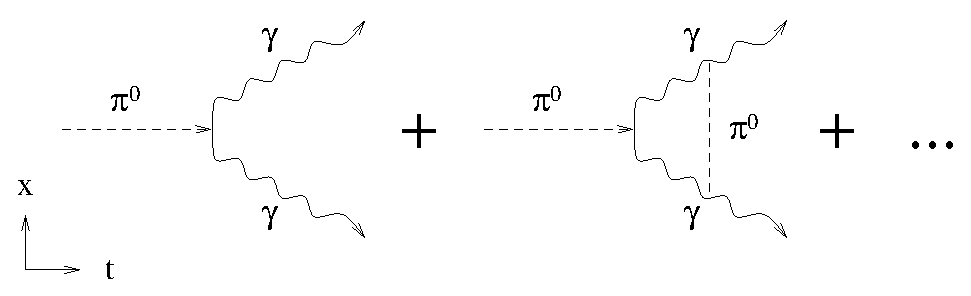
\includegraphics[width=0.6\linewidth]{fig4.eps}
\end{center}
Calculating the probability of the initial-to-final-state process
involves sums over all such configurations, as well as integrations
over all intermediate momenta, and these diagrams help organize the
calculation.  Moreover, if the coupling is weak (as it is for
electrodynamics, the weak nuclear force, and the strong nuclear force
at large energies), the series of diagrams is geometric, and a
calculation may be truncated after a few of them.

The nuclear strong force at low energies (such as the mass of the
proton) doesn't have this property.  To calculate low-energy strong
force processes, theorists numerically evaluate path integrals on a
computer by first discretizing it to a lattice.  In my thesis, I
measure a process calculated that way, as a test of the calculation.

\end{document}
